%
% ─── CAPITULO 7: INTRODUCCION AL RAY TRACING ────────────────────────────────────
%

En los anteriores capítulos hemos visto cómo asignar colores a los píxeles utilizando el fragment shader y cómo dibujar hermosos fractales en la superficie que ocupan dos triángulos. Sin embargo, no hemos podido movernos de las dos dimensiones. Esto se debe a la dificultad que de por sí supone que en 2D un píxel puede representar un único punto del plano mientras que en 3D un píxel representa infinitos puntos del espacio. Nuestro objetivo ahora es poder visualizar escenas simples en 3D para posteriormente renderizar fractales en 3D.

\section{Definición de Ray-Tracing}

En el mundo de la informática gráfica existen dos formas fundamentales de proceder al renderizado de escenas. Supongamos que tenemos una escena 3D con varios objetos, como pueden ser por ejemplo un cubo y un par de esferas y queremos visualizar la misma en un canvas 2D.
\begin{itemize}
    \item Una de las formas de renderizarlo es identificar para cada objeto (también llamado primitiva) qué píxeles ocupan y asignar color a cada píxel, aplicando posibles modelos de iluminación y texturas. Esta es la técnica conocida como \textbf{rasterización}.
    \item Otra forma es, para cada pixel, calcular qué primitivas ocupan posiciones del espacio asociadas a dicho píxel y colorearlo dependiendo de la primitiva más cercana al observador. Esta es la base del \textbf{Ray-Tracing}.
\end{itemize}

Más en profundidad, la idea es situar al espectador en una cierta posición de la escena y colocar frente a él un plano, el cual estará dividido en tantos píxeles como tenga el canvas, de tal manera que se `trazan rayos' que salen desde la posición del espectador en dirección a cada píxel, por lo que se lanzan tantos rayos como píxeles haya. El rayo atraviesa el plano y avanza por la escena hasta que encuentra la intersección con un objeto. En este caso, se calcula en qué punto se ha alcanzado la intersección y se evalúa un modelo de iluminación o se asigna un color dependiendo de las características de la escena. también es posible que el rayo no alcance ningún objeto y se pierda, en cuyo caso habría que saber qué hacer con los píxeles cuyos rayos se pierden en el infinito. En la imagen \ref{fig:RT} se puede observar un esquema aclarativo del funcionamiento de este método.

\begin{figure} [ht]
    \centering
    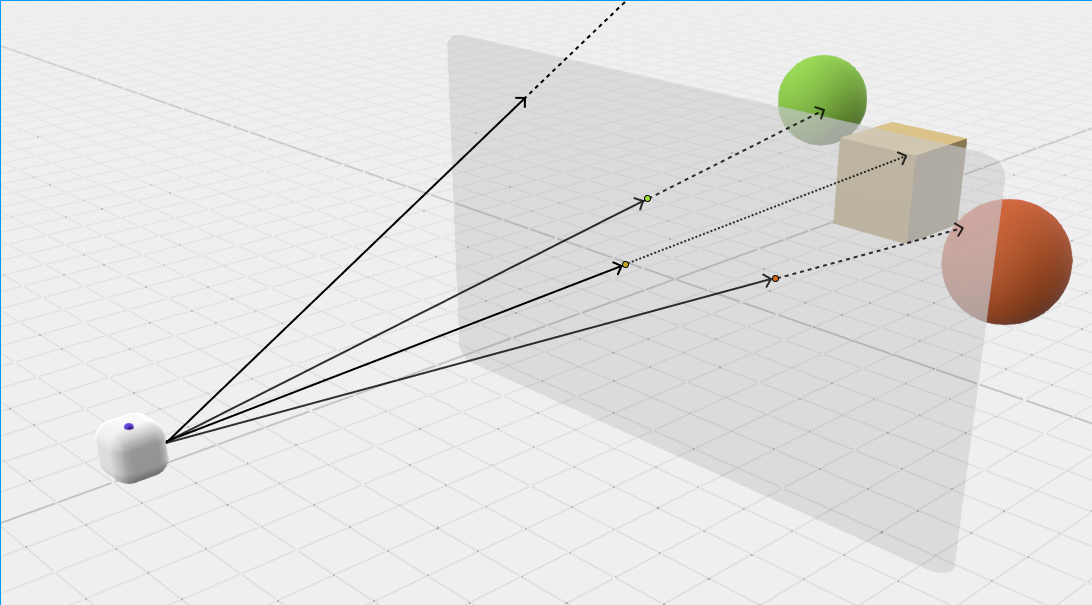
\includegraphics[scale = 0.4]{img/C7/RT.png}
    \caption{Esquema básico del funcionamiento del Ray-Tracing}
    \label{fig:RT}
\end{figure}

La principal ventaja que tiene el Ray-Tracing (en adelante RT) sobre la rasterización es que este trazado de rayos nos permite facilitar el cálculo de los reflejos y sombras creados por las iluminaciones del entorno, consiguiendo así efectos mucho más realistas en las escenas. Además, recordemos que las figuras fractales que perseguimos no es posible dibujarlas mediante un conjunto de vértices o aristas al no ser objetos de la geometría euclídea, por lo que sería muy difícil expresarlos como primitivas rasterizables. Lo más natural es lanzar rayos y, en caso de detectar intersección con el fractal estimar la normal en dicho punto y aplicar un modelo de iluminación. Es por esta serie de razones por las que para nuestro objetivo necesitamos programar un \textit{ray-tracer} inicialmente básico con el objetivo futuro de renderizar fractales 3D.

Sin embargo, este algoritmo tiene una principal desventaja, y es que es un proceso muy costoso, y más aún cuanto más detalle queramos conseguir. Es por esto que ha sido muy difícil dar el salto al ray tracing en tiempo real. Por ejemplo, en el mundo de los videojuegos, NVIDIA, que es una famosa empresa desarrolladora de tarjetas gráficas, comenzó a desarrollar algoritmos para poder utilizar RT en sus tarjetas hace varios años, pero hasta finales de 2018 no salieron las primeras gráficas con estas características al mercado. Por su parte, los juegos también deben soportar el algoritmo, por lo que aún son una minoría de videojuegos los que en la actualidad soportan Ray Tracing. En un futuro no muy lejano es posible que haya una tendencia a un desarrollo masivo de juegos que utilicen RT, pero de momento solo tenemos algunos ejemplos como Battlefield V, Minecraft, Metro Exodus, Watch Dogs y Call of Duty: Modern Warfare (2019).

Sin embargo, a pesar de dicha desventaja veremos que nuestro código puede ejecutarse en tiempo real, teniendo en cuenta siempre que debemos evitar el uso de funciones que comprometan la velocidad de ejecución. Por ejemplo, la función \verb|pow| es muy lenta, por lo que debemos evitar usarla cuando se usen potencias enteras.



